\subsection{实验目的-MySQL 日志}
了解 MySQL 日志.
%
\subsection{实验原理}
日志是 mysql 数据库的重要组成部分。日志文件中记录着 mysql 数据库运行期间发生的变化,
也就是说用来记录 mysql 数据库的客户端连接状况、SQL 语句的执行情况和错误信息等。当
数据库遭到意外的损坏时,可以通过日志查看文件出错的原因,并且可以通过日志文件进
行数据恢复。
%
\subsection{实验环境}
Kali Linux:192.168.1.2 hydra
CentOS6.5:192.168.1.3 MySQL
%
\subsection{实验步骤}
\subsubsection{破解mysql的root密码,并抓取破解数据包}
在实验开始前先开启 CentOS6.5 上的通用日志。
在 kali linux 的终端中输入命令``wireshark'',回车,打开 wireshark。
\begin{figure}[H]
  \begin{center}
    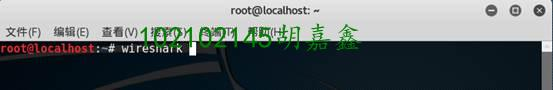
\includegraphics[width=0.40\textwidth]{2_12_1.jpeg}
  \end{center}
\end{figure}

在打开的 wireshark 中选择要监听的网卡,单击``开始捕获分组''按钮,
开始进行抓包。
\begin{figure}[H]
  \begin{center}
    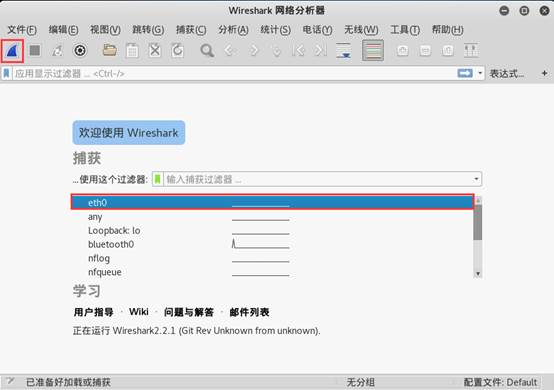
\includegraphics[width=0.40\textwidth]{2_12_2.jpeg}
  \end{center}
\end{figure}

重新打开一个终端,输入命令
\begin{minted}[bgcolor=bg,breaklines=true]{sh}
cd /root/桌面
cat userlist.txt
cat passlist.txt
\end{minted}
查看用户名文件和密码文件。
\begin{figure}[H]
  \begin{center}
    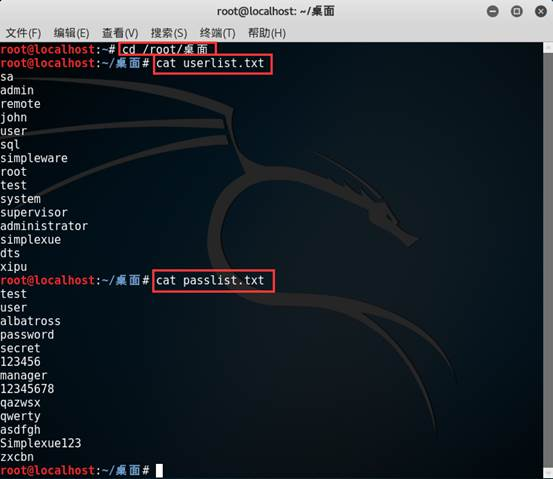
\includegraphics[width=0.40\textwidth]{2_12_3.jpeg}
  \end{center}
\end{figure}

在终端输入命令
\begin{minted}[bgcolor=bg,breaklines=true]{sh}
hydra -L userlist.txt -P passlist.txt 192.168.1.3 mysql -t 1
\end{minted}
开始破解 mysql。
这里为了便于后面的数据包分析,将线程数设置为 1。
\begin{figure}[H]
  \begin{center}
    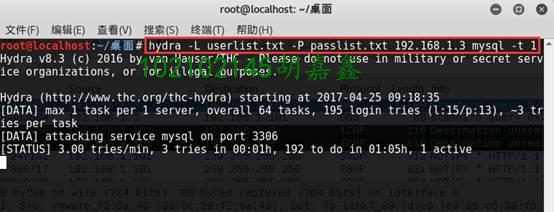
\includegraphics[width=0.40\textwidth]{2_12_4.jpeg}
  \end{center}
\end{figure}

在破解的过程中发现耗时估计会很长,请耐心等待。这里我们为了便于分析,
新建并简化用户名文件和密码文件。
\begin{figure}[H]
  \begin{center}
    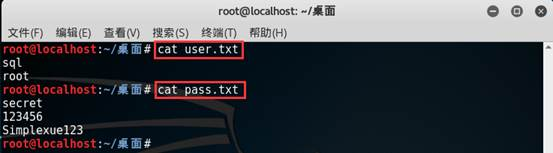
\includegraphics[width=0.40\textwidth]{2_12_5.jpeg}
  \end{center}
\end{figure}

重新开始抓包,在终端输入命令
\begin{minted}[bgcolor=bg,breaklines=true]{sh}
hydra -L user.txt -P pass.txt 192.168.1.3 mysql -t 1
\end{minted}
开始破解 mysql。
\begin{figure}[H]
  \begin{center}
    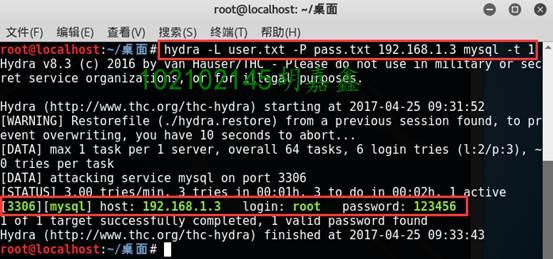
\includegraphics[width=0.40\textwidth]{2_12_6.jpeg}
  \end{center}
\end{figure}

wireshark 停止抓包,过滤端口为 3306 的数据包。
\begin{figure}[H]
  \begin{center}
    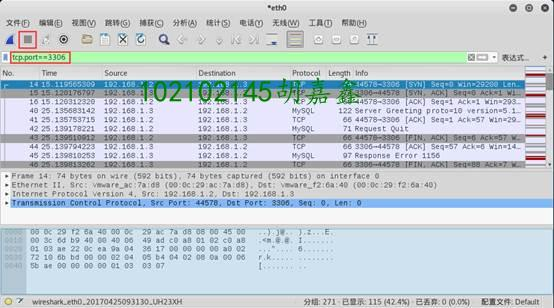
\includegraphics[width=0.40\textwidth]{2_12_7.jpeg}
  \end{center}
\end{figure}
%
\subsubsection{分析抓取的数据包,理解 mysql 破解过程}
通过观察 wireshark 抓取的数据包可知,wireshark 已经对抓取的数据包使用
``[''的符号对连接建立、传输数据、断开连接的过程进行了标识。
\begin{figure}[H]
  \begin{center}
    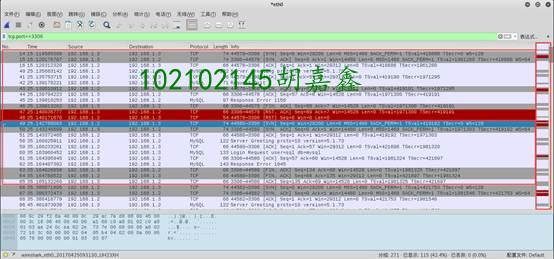
\includegraphics[width=0.40\textwidth]{2_12_8.jpeg}
  \end{center}
\end{figure}

下面我们对其中一个过程的数包进行分析。首先查看第一个数据包,
源地址为 \texttt{192.168.1.2},源端口为 \texttt{44578},目的地址为\texttt{192.168.1.3},
目的端口为 \texttt{3306},TCP 序号为 SYN,且置为 $1$,
表示客户端 \texttt{192.168.1.2} 向服务器 \texttt{192.168.1.3} 发送了一个连接请求报文。
\begin{figure}[H]
  \begin{center}
    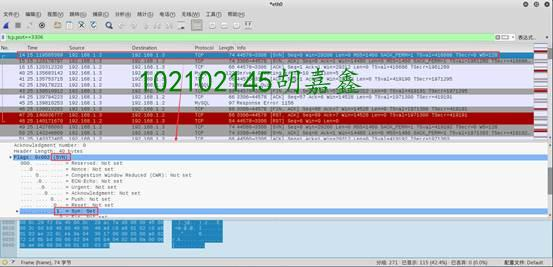
\includegraphics[width=0.40\textwidth]{2_12_9.jpeg}
  \end{center}
\end{figure}

再查看第二个数据包,
\texttt{192.168.1.3} 收到请求后确认联机信息,向 \texttt{192.168.1.2} 发送数据包,
SYN 置为 $1$,ACK 也置为 $1$。
\begin{figure}[H]
  \begin{center}
    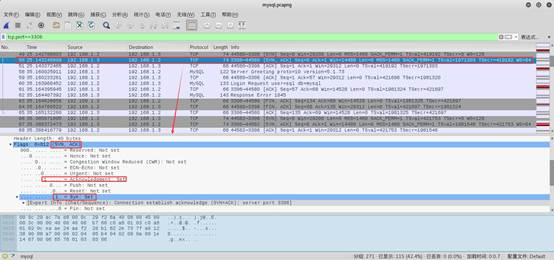
\includegraphics[width=0.40\textwidth]{2_12_10.jpeg}
  \end{center}
\end{figure}

查看第三个数据包,主机 \texttt{192.168.1.2} 收到数据包后检查无误,
向 \texttt{192.168.1.3} 发送数据包,
ACK 置为 $1$,至此三次握手完毕,连接建立,后面就可以开始传输数据了。
\begin{figure}[H]
  \begin{center}
    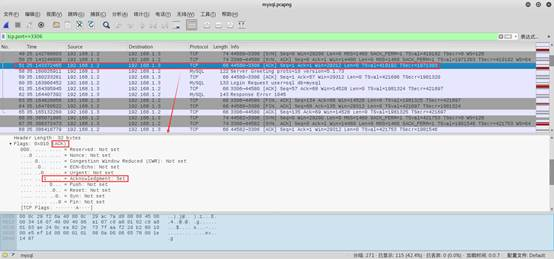
\includegraphics[width=0.40\textwidth]{2_12_11.jpeg}
  \end{center}
\end{figure}

从这个数据包信息可知,mysql 的版本为 \texttt{5.1.73}。
\begin{figure}[H]
  \begin{center}
    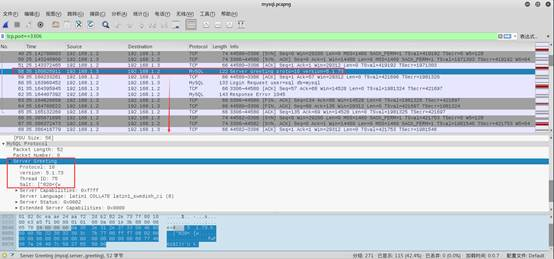
\includegraphics[width=0.40\textwidth]{2_12_12.jpeg}
  \end{center}
\end{figure}

查看这个数据包,可以看到传输的数据,即 mysql 登录信息,用户名为 sql,
表明正在破解 mysql。
由上一步骤的数据包信息可
知 mysql 对密码进行了加盐。
\begin{figure}[H]
  \begin{center}
    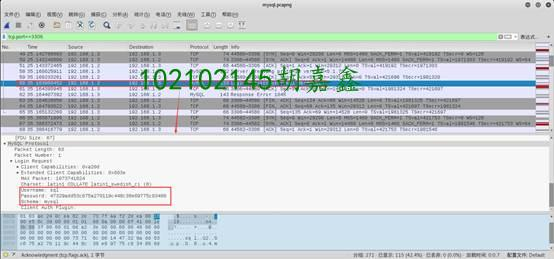
\includegraphics[width=0.40\textwidth]{2_12_13.jpeg}
  \end{center}
\end{figure}

查看 Response,可以看到为 Error,说明连接不成功,即用户名或者密码错误。
之后则是连接的结束过程。
\begin{figure}[H]
  \begin{center}
    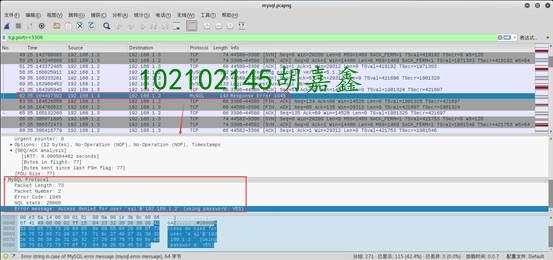
\includegraphics[width=0.40\textwidth]{2_12_14.jpeg}
  \end{center}
\end{figure}

我们找到破解出来的 root 密码对应的数据包,
并查看其 response 数据包,发现与其它 response 数据包相比,
为 OK。
\begin{figure}[H]
  \begin{center}
    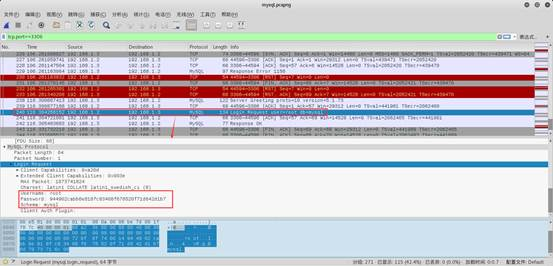
\includegraphics[width=0.40\textwidth]{2_12_15.jpeg}
  \end{center}
\end{figure}
\begin{figure}[H]
  \begin{center}
    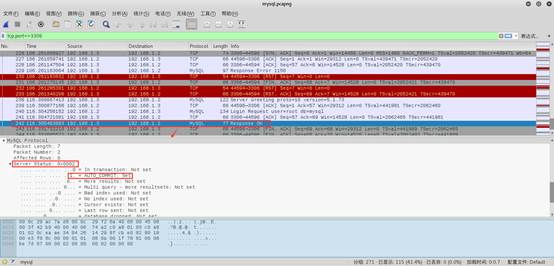
\includegraphics[width=0.40\textwidth]{2_12_16.jpeg}
  \end{center}
\end{figure}
%
\subsubsection{查看 mysql 通用日志}
在 CentOS6.5 上打开终端,输入命令
\begin{minted}[bgcolor=bg,breaklines=true]{sh}
service mysqld start
mysql -u root -p
# 密码 123456
\end{minted}
\begin{figure}[H]
  \begin{center}
    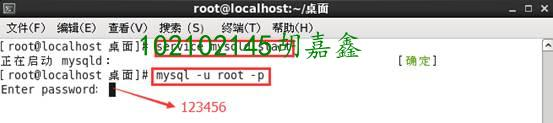
\includegraphics[width=0.40\textwidth]{2_12_17.jpeg}
  \end{center}
\end{figure}

在 mysql 中输入命令
\begin{minted}[bgcolor=bg,breaklines=true]{sh}
set global general_log = on;
\end{minted}
开启通用日志,再输入命令
\begin{minted}[bgcolor=bg,breaklines=true]{sh}
show global variables like '%genera%';
\end{minted}
进行查看,可以看到通用日志已开启。
\begin{figure}[H]
  \begin{center}
    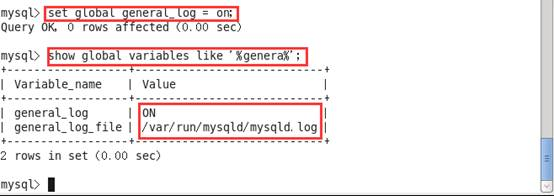
\includegraphics[width=0.40\textwidth]{2_12_18.jpeg}
  \end{center}
\end{figure}

在终端输入命令
\begin{minted}[bgcolor=bg,breaklines=true]{sh}
cat /var/run/mysqld/mysqld.log
\end{minted}
查看到前面破解过程的 mysql 登录
信息。
\begin{figure}[H]
  \begin{center}
    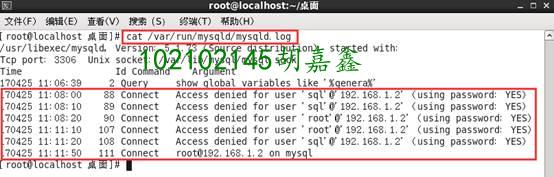
\includegraphics[width=0.40\textwidth]{2_12_19.jpeg}
  \end{center}
\end{figure}
